\chapter{Partitioning}

\textbf{Partitioning} becomes necessary when dealing with \textbf{large data sets} and high \textbf{query throughput}. It is a technique that divides a large data set into smaller, more manageable parts. This is done to improve the performance of the system. Partitioning can be done in various ways, such as horizontal partitioning, vertical partitioning, and functional partitioning. In this chapter, we will discuss the different types of partitioning and their benefits.

``Partition'' is the most common term, but it may vary depending on the technology:
\begin{itemize}
   \item \textbf{Shard} in MongoDB, Elasticsearch, and Cassandra.
   \item \textbf{Region} in HBase.
   \item \textbf{VBucket} in Couchbase.
   \item \textbf{Tablet} in Bigtable.
   \item \textbf{VNode} in Riak and Cassandra.	
\end{itemize} 

\section{Partitioning concepts}
First, partitions must be \textbf{defined}, in the sense that each piece of data must be assigned to a partition. This can be done in various ways, such as hashing, range partitioning, or list partitioning.

Then, each partition should have its own \textbf{characteristics}, i.e. should support a known set of operations, since it acts as a small per se database.

Clearly, different partitions may reside on different nodes, enabling scalability.


\subsection{Combining partitioning with replication}

\begin{paracol}{2}
   \colfill
   Partitioning can be combined with replication to improve the performance and reliability of the system. Replication is the process of creating multiple copies of the data and storing them on different nodes. This ensures that the data is available even if one of the nodes fails. \ul{By combining partitioning with replication, you can achieve high availability and fault tolerance.}
   \colfill
   
   \switchcolumn

   \begin{figure}[htbp]
      \centering
      \includegraphics[width=0.95\columnwidth]{images/11/leader_follower.png}
      \caption{Leader-follower model}
      \label{fig:11/leader_follower}
   \end{figure}
\end{paracol}

This can be achieved in various ways:
\begin{enumerate}
   \item Node Storage of Multiple Partitions
   \begin{itemize}
      \item Nodes can store more than one partition, and \ul{each partition can be stored on multiple nodes}.
   \end{itemize}
   \item \textbf{Leader} and \textbf{Follower} assignment
   \begin{itemize}
      \item Each node stores a partition, and one of the nodes is designated as the leader. The leader is responsible for handling all write operations, while the followers, assigned to different nodes, replicate the data from the leader.
   \end{itemize}
   \item Replication and Partitioning
   \begin{itemize}
      \item The two techniques are enforced independently.
   \end{itemize}
\end{enumerate}

The Goal of partitioning is to spread data and query load \textbf{evenly} among the nodes.
Unfair partitioning can lead to \textbf{hot spots}, where some nodes are overloaded while others are underutilized.\\
Randomizing the partitioning function can help to avoid hot spots, but it can also make it difficult to locate data, requiring to query all nodes to get a value.

\subsection{Key-Range Partitioning}
A first improvement might be to provide a range-key assignment allowing to locate data, as it happens in libraries, where books are ordered by author or title.\\
In this way you know the boundaries of where to search. This is very easy to implement and to understand,
however, it is \textit{not} optimal:
\ul{data may \textbf{not} be evenly distributed among the possible keys}.

Consider partitioning a student database by student ID. If student IDs are assigned sequentially, then all students enrolled in the same year will have similar IDs. This can lead to uneven distribution of data across partitions, as students from the same year may be assigned to the same partition, while other partitions may be underutilized.

\section{Avoiding Hot spots}
So with key-range partitioning, the problem is that some keys may be more popular than others due to access patterns, leading to hot spots.\\
In, for instance, a sensor database, all today's writes would end up in the same ``today's partition'', while the rest of the partitions would be idle.
\nl

A solution might be to change-key structure, for instance by adding a prefix to the key, such as the sensor ID, to distribute the data more evenly.

\subsection{Hash partitioning}
A better solution is to use \textbf{hash partitioning}, where a hash function is used to map keys to partitions.\\
However we must be careful because \textbf{inconsistent} hashing can lead to hot spots, as the hash function may not distribute keys evenly.
In general, however, a good hash function will make skewed data uniformly distributed across partitions.

Note also that hash partitioning is very bad for range queries, as even similar data is spread randomly across the partitions.\\
In Cassandra, a \textbf{compound primary key} is used, where the first part is hashed to determine the partition, while the second part is an index used to order data within the partition, allowing for efficient range queries within a partition.\\
Range queries on the first column (the hashed one) are not possible, as data is spread randomly across partitions, so all partitions must be queried in such case.

\subsubsection{Secondary Indexes}
% Copilot generated
Secondary indexes are a way to avoid hot spots in hash partitioning.\\
The idea is to create a separate index that maps the secondary key to the primary key, and then use the primary key to locate the data.\\
This way, the secondary key is hashed and distributed evenly across the partitions, while the primary key is used to locate the data.


\begin{itemize}
   \item \textbf{Document}-based partitioning (local indexes)
   \begin{itemize}
      \item Each listing has a unique document ID
      \item Database is partitioned based on the document ID
      \item Secondary indexes are on fields like color and make
      \item Each partition maintains its own secondary indexes
      \item \ul{\textit{Reading} requires querying all partitions}
   \end{itemize}
   \item \textbf{Term}-based partitioning (global indexes)\\
   The ``term'' is essentially the value of the indexed field.
   \begin{itemize}
      \item A Global index covers data in all partitions.
      \item Partitioning is based on the term ID, which is not the primary key index.
      \item Example: Colors a-r in partition 1, s-z in partition 2.
      \item A single entry in secondary index may include records from all primary key partitions.
      \item Term determines the partition of the index
      \item The Term concept comes from full-text indexes
   \end{itemize}
\end{itemize}

Global index allows clients to request specific partitions, and avoids scatter/gather over all partitions, so read operations are more efficient.
However, write operations become more complex, as the write to a document may require updating multiple partitions, both the document partition and the index partition.
Besides, each term in a document could be on a different partition, leading to multiple writes for a single document update.

\paragraph{Detailed Comparison: Document-Based vs Term-Based}

Consider a database of used car listings with:
\begin{itemize}
   \item \textbf{Primary key}: \texttt{document\_id} (unique listing ID)
   \item \textbf{Secondary indexes}: \texttt{color}, \texttt{make} (brand), \texttt{model}
   \item Database partitioned by \texttt{document\_id}
\end{itemize}

\subparagraph{Document-Based Partitioning (Local Indexes)}
Each partition maintains its \textbf{own local secondary indexes} only for the documents it contains.

\begin{lstlisting}[language=bash, basicstyle=\footnotesize\ttfamily]
Partition 0 (document_id: 0-499):
|- Documents: {id:0, color:red}, {id:1, color:blue}, ...
`- Local Index:
   |- color:red -> [0, 23, 145, ...]
   |- color:blue -> [1, 67, 234, ...]
   `- make:toyota -> [12, 89, ...]

Partition 1 (document_id: 500-999):
|- Documents: {id:500, color:red}, {id:501, color:green}, ...
`- Local Index:
   |- color:red -> [500, 678, 891, ...]
   |- color:green -> [501, 602, ...]
   `- make:toyota -> [534, 712, ...]
\end{lstlisting}

\textbf{Query example (scatter/gather)}:
\begin{lstlisting}[language=bash, basicstyle=\footnotesize\ttfamily]
Query: "SELECT * WHERE color='red'"
  |-> Partition 0: [0, 23, 145]
  |-> Partition 1: [500, 678, 891]
  |-> Partition 2: [1001, 1234]
  `-> Partition 3: [1500, 1789]
       |
       v
  Merge results: [0, 23, 145, 500, 678, 891, 1001, 1234, 1500, 1789]
\end{lstlisting}

\checkmark \textbf{Write}: Simple - updates only the partition containing the document\\
\xmark \textbf{Read}: Complex - must query \textbf{all} partitions and merge results

\subparagraph{Term-Based Partitioning (Global Indexes)}
A single \textbf{global index} for each secondary field, partitioned by term (field value).

\begin{lstlisting}[language=bash, basicstyle=\footnotesize\ttfamily]
Global Index for "color" (partitioned by term):
Partition A (colors: a-m):
  |- blue -> [doc:1, doc:67, doc:234, doc:501, ...]
  |- green -> [doc:501, doc:602, ...]
  `- black -> [doc:34, doc:456, ...]

Partition B (colors: n-z):
  |- red -> [doc:0, doc:23, doc:145, doc:500, doc:678, ...]
  |- white -> [doc:89, doc:345, ...]
  `- yellow -> [doc:123, doc:789, ...]
\end{lstlisting}

\textbf{Note}: Document IDs in indexes can come from \textbf{any partition} of the main database!

\textbf{Query and write examples}:
\begin{lstlisting}[language=bash, basicstyle=\footnotesize\ttfamily]
Query: "SELECT * WHERE color='red'"
  `-> Global Index Partition B (red falls in n-z)
       `-> Returns: [doc:0, doc:23, doc:145, doc:500, doc:678, ...]

INSERT {id:1500, color:'red', make:'toyota'}
  |-> Database Partition 3 (for doc_id=1500)
  |-> Global Index "color" Partition B (for term='red')
  `-> Global Index "make" Partition X (for term='toyota')
\end{lstlisting}

\checkmark \textbf{Read}: Efficient - query goes to a single index partition\\
\xmark \textbf{Write}: Complex - may update multiple partitions (document + multiple index partitions)

\subparagraph{Trade-offs Summary}

\begin{table}[htbp]
\centering
\footnotesize
\begin{tabular}{|l|c|c|}
\hline
\textbf{Aspect} & \textbf{Document-Based} & \textbf{Term-Based} \\
\hline
Read & Slow (scatter/gather) & Fast (single partition) \\
Write & Simple (single partition) & Complex (multiple partitions) \\
Consistency & Easier (local) & Harder (distributed) \\
Complexity & Low & High \\
Best for & Write-heavy workload & Read-heavy workload \\
\hline
\end{tabular}
\caption{Document-Based vs Term-Based Secondary Index Partitioning}
\label{tab:11/secondary-indexes-comparison}
\end{table}

\textbf{Use Document-Based when}: Writes are more frequent than reads, secondary index queries are rare. Example: logging system.

\textbf{Use Term-Based when}: Reads are more frequent than writes, secondary index queries are common. Example: e-commerce with searches by color/brand.

\subparagraph{Analogy}
\begin{itemize}
   \item \textbf{Document-Based}: Like having a library in each city with its own catalog. To find all ``Hemingway'' books, you must check every city's library catalog.
   \item \textbf{Term-Based}: Like having a national catalog partitioned by author (A-M, N-Z). To find ``Hemingway'' go directly to the H partition, but when adding a new book you must update both the local library and the national catalog.
\end{itemize}

\subparagraph{Visual Comparison}

\begin{figure}[htbp]
\centering
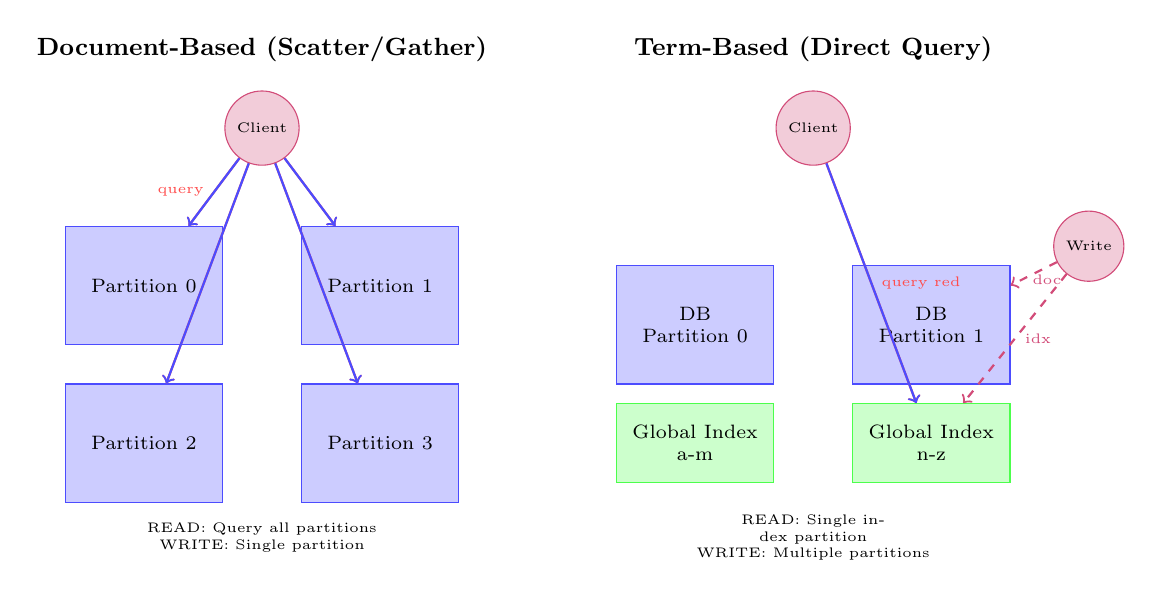
\begin{tikzpicture}[
   node distance=0.8cm,
   partition/.style={rectangle, draw=blue!70, fill=blue!20, minimum width=2cm, minimum height=1.5cm, text centered, font=\scriptsize, align=center},
   index/.style={rectangle, draw=green!70, fill=green!20, minimum width=2cm, minimum height=1cm, text centered, font=\scriptsize, align=center},
   client/.style={circle, draw=purple!70, fill=purple!20, minimum size=0.8cm, text centered, font=\tiny},
   queryarrow/.style={->, thick, red!70},
   writearrow/.style={->, thick, dashed, purple!70},
   responsearrow/.style={<-, thick, blue!70}
]

% Document-Based (Left side)
\node[client] (client1) at (0,4) {Client};
\node[partition] (p0) at (-1.5,2) {Partition 0};
\node[partition] (p1) at (1.5,2) {Partition 1};
\node[partition] (p2) at (-1.5,0) {Partition 2};
\node[partition] (p3) at (1.5,0) {Partition 3};

% Query arrows
\draw[queryarrow] (client1) -- (p0) node[midway, left, font=\tiny] {query};
\draw[queryarrow] (client1) -- (p1);
\draw[queryarrow] (client1) -- (p2);
\draw[queryarrow] (client1) -- (p3);

% Response arrows (simplified)
\draw[responsearrow] (p0) -- (client1);
\draw[responsearrow] (p1) -- (client1);
\draw[responsearrow] (p2) -- (client1);
\draw[responsearrow] (p3) -- (client1);

\node[font=\small\bfseries] at (0,5) {Document-Based (Scatter/Gather)};
\node[font=\tiny, text width=3cm, align=center] at (0,-1.2) {READ: Query all partitions\\WRITE: Single partition};

% Term-Based (Right side)
\node[client] (client2) at (7,4) {Client};

% Database partitions
\node[partition] (db0) at (5.5,1.5) {DB\\Partition 0};
\node[partition] (db1) at (8.5,1.5) {DB\\Partition 1};

% Global index partitions
\node[index] (idx0) at (5.5,0) {Global Index\\a-m};
\node[index] (idx1) at (8.5,0) {Global Index\\n-z};

% Read query (goes only to index)
\draw[queryarrow] (client2) -- (idx1) node[midway, right, font=\tiny, text width=1cm, align=center] {query red};
\draw[responsearrow] (idx1) -- (client2);

% Write operation (goes to multiple places)
\node[client] (writer) at (10.5,2.5) {\tiny Write};
\draw[writearrow] (writer) -- (db1) node[near end, right, font=\tiny] {doc};
\draw[writearrow] (writer) -- (idx1) node[midway, right, font=\tiny] {idx};

\node[font=\small\bfseries] at (7,5) {Term-Based (Direct Query)};
\node[font=\tiny, text width=3cm, align=center] at (7,-1.2) {READ: Single index partition\\WRITE: Multiple partitions};

\end{tikzpicture}
\caption{Visual comparison of Document-Based vs Term-Based partitioning query patterns}
\label{fig:11/secondary-index-comparison}
\end{figure}

\begin{figure}[htbp]
\centering
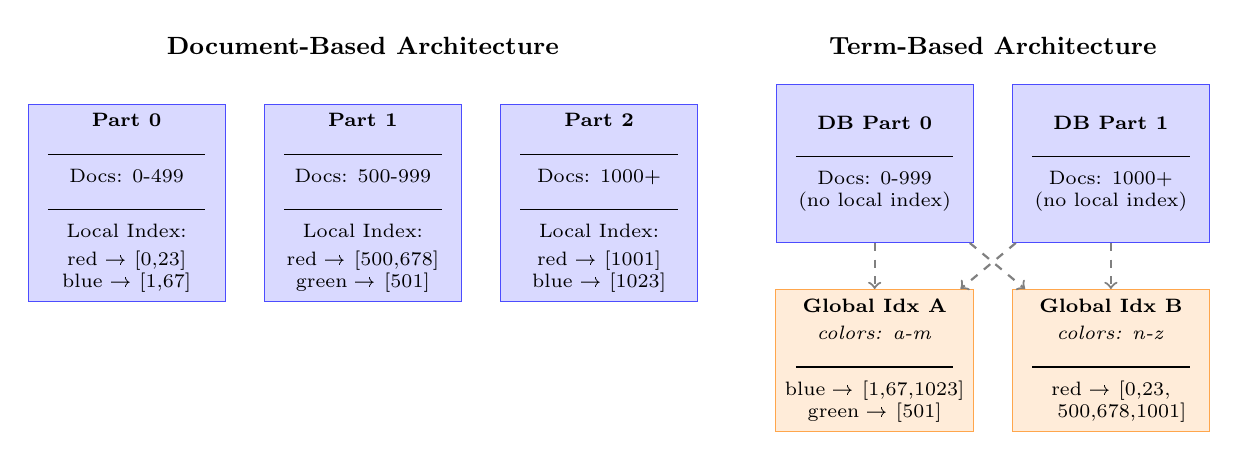
\begin{tikzpicture}[
   node distance=0.5cm,
   dbpart/.style={rectangle, draw=blue!70, fill=blue!15, minimum width=2.5cm, minimum height=2cm, text centered, font=\scriptsize, align=center},
   globalidx/.style={rectangle, draw=orange!70, fill=orange!15, minimum width=2.5cm, minimum height=1.5cm, text centered, font=\scriptsize, align=center},
   data/.style={font=\tiny, align=left}
]

% Document-Based architecture
\node[font=\small\bfseries] at (0,4.5) {Document-Based Architecture};

\node[dbpart] (d0) at (-3,2.5) {
   \textbf{Part 0}\\[2pt]
   \rule{2cm}{0.4pt}\\[2pt]
   Docs: 0-499\\[2pt]
   \rule{2cm}{0.4pt}\\[2pt]
   Local Index:\\[2pt]
   red → [0,23]\\
   blue → [1,67]
};

\node[dbpart] (d1) at (0,2.5) {
   \textbf{Part 1}\\[2pt]
   \rule{2cm}{0.4pt}\\[2pt]
   Docs: 500-999\\[2pt]
   \rule{2cm}{0.4pt}\\[2pt]
   Local Index:\\[2pt]
   red → [500,678]\\
   green → [501]
};

\node[dbpart] (d2) at (3,2.5) {
   \textbf{Part 2}\\[2pt]
   \rule{2cm}{0.4pt}\\[2pt]
   Docs: 1000+\\[2pt]
   \rule{2cm}{0.4pt}\\[2pt]
   Local Index:\\[2pt]
   red → [1001]\\
   blue → [1023]
};

% Term-Based architecture
\node[font=\small\bfseries] at (8,4.5) {Term-Based Architecture};

\node[dbpart] (t0) at (6.5,3) {
   \textbf{DB Part 0}\\[2pt]
   \rule{2cm}{0.4pt}\\[2pt]
   Docs: 0-999\\
   (no local index)
};

\node[dbpart] (t1) at (9.5,3) {
   \textbf{DB Part 1}\\[2pt]
   \rule{2cm}{0.4pt}\\[2pt]
   Docs: 1000+\\
   (no local index)
};

\node[globalidx] (gi0) at (6.5,0.5) {
   \textbf{Global Idx A}\\[2pt]
   \textit{colors: a-m}\\[2pt]
   \rule{2cm}{0.4pt}\\[2pt]
   blue → [1,67,1023]\\
   green → [501]
};

\node[globalidx] (gi1) at (9.5,0.5) {
   \textbf{Global Idx B}\\[2pt]
   \textit{colors: n-z}\\[2pt]
   \rule{2cm}{0.4pt}\\[2pt]
   red → [0,23,\\
   \quad 500,678,1001]
};

% Arrows showing relationships
\draw[->, thick, gray, dashed] (t0) -- (gi0);
\draw[->, thick, gray, dashed] (t0) -- (gi1);
\draw[->, thick, gray, dashed] (t1) -- (gi0);
\draw[->, thick, gray, dashed] (t1) -- (gi1);

\end{tikzpicture}
\caption{Data distribution in Document-Based vs Term-Based secondary index partitioning}
\label{fig:11/secondary-index-architecture}
\end{figure}

\section{Rebalancing}
Rebalancing is the process of moving data between partitions to ensure that the data is evenly distributed among the nodes. This is necessary when the data distribution changes, for example, when new nodes are added to the system or when the data distribution becomes uneven due to hot spots. Rebalancing can be done in various ways, such as automatic rebalancing, manual rebalancing, and dynamic rebalancing.

\framedt{Challenges in rebalancing}{
   \begin{itemize}
      \item Fair load distribution
      \item Continuous operation during rebalancing
      \item Minimizing data movement
   \end{itemize}
}

\begin{itemize}
   \item \textbf{Automatic} rebalancing - System automatically rebalances the data when necessary without any human intervention.
   May be unpredictable and expensive, but requires less maintanance.
   \item \textbf{Manual} rebalancing - Administrator manually rebalances the data when necessary. May be better since and admin may have a more \textit{comprehensive} view of the distributed system, while a machine may be limited by network partitioning, discovery, etc.
   \item \textbf{Hybrid} approach - Combines automatic and manual rebalancing. The system automatically rebalances the data when necessary, but the administrator can override the system's decisions. 
\end{itemize}


\subsection{Techniques}

A common approach to address rebalancing is the ``\textbf{Hash mod N}'' strategy, where each key is hashed and then the modulo operation with the number of nodes (N) determines the partition. However, this approach can lead to significant data movement when nodes are added or removed, as all keys need to be rehashed.

\framedt{Optimizing rebalancing - Kademlia and P2P recalls}{
Assigning keys to nodes computing $h(key) \bmod \#\{\text{nodes}\} \rightarrow \text{node}$ is intuitive but leads to a tremendous amount of data movement when nodes are added or removed, since all modulo values must be recomputed.\\
A better solution is to use a \textbf{distributed hash table} (DHT) such as \textbf{Kademlia} or \textbf{Chord}, which allows to find the node responsible for a key in $O(\log n)$ steps.

\textbf{Kademlia's approach}: Both nodes and keys are hashed into the same fixed identifier space (e.g., 160-bit). Each key is stored on the node whose ID is \textit{closest} to the key's hash, measured by XOR distance: $d(a,b) = a \oplus b$. When nodes join/leave, only keys in their immediate XOR neighborhood need to be transferred, minimizing data movement.

\textit{Example}: If key hash is \texttt{101101} and node IDs are \texttt{101100}, \texttt{110001}, \texttt{101111}, the key goes to \texttt{101100} (XOR distance = 1, the smallest).

The key intuition exploited by both Kademlia and Chord is to \textbf{fix the granularity of the keyspace prior to partitioning}. By pre-defining a large identifier space (e.g., $2^{160}$ possible IDs), adding or removing nodes only affects a small fraction of keys, as the keyspace boundaries remain constant.
}


Another idea is to have many \textbf{fixed partitions}, more than nodes, and assigning several (like 1000) partitions to each node. When a node is added it steals partitions from other nodes, and when a node is removed its partitions are reassigned to other nodes. This way, only a small portion of the data needs to be moved during rebalancing.
Partitions are never split or merged, only reassigned. Clearly, we can exploit more powerful nodes to hold more partitions.\\
The issue with this is that incorrect boundaries can lead to hot spots, so careful monitoring is required.

\textbf{Dynamic Partitioning} is another approach, where partitions can be split or merged based on the data distribution. This allows for more flexibility in rebalancing, as partitions can be adjusted to better fit the data distribution. However, this approach can be more complex to implement and manage.\\
Partitions are split when they exceed a configured size, and merged when some other gets deleted.\\
Each partition assigned to one node.

\textbf{Proportional Partitioning} may be enforced in different fashions:
\begin{itemize}
   \item Dynamic Partitioning - Number of partitions varies is proportional to dataset size.
   Splitting and merging processes maintain partition size.
   \item Fixed Number of Partitions - the number of partitions is fixed and proportional to dataset size, it is independent of the number of nodes.
   \item Proportional Assignment to Nodes - Number of partitions proportional to number of nodes
\end{itemize}
This allows for better utilization of resources, as more powerful nodes can handle more partitions. However, this approach requires careful monitoring and management to ensure that the data is evenly distributed among the nodes.

% \framedt{Automatic vs Manual Rebalancing}{
%    With automatic rebalancing the system automatically rebalances the data when necessary without any human intervention.
%    May be unpredictable and expensive, but requires less maintanance.
%    \nl

%    With manual rebalancing the administrator manually rebalances the data when necessary. May be better since and admin may have a more \textit{comprehensive} view of the distributed system, while a machine may be limited by network partitioning, discovery, etc.
%    This is considerably slower but may prevent operational surprises.
% }

\subsection{Routing and Querying}
Routing is the process of determining which partition to send a query to. This is done by either forwarding requests to a routing tier, or by having partition-aware clients which know how the data is distributed. Alternatively, client and also query any node, if there is no routing tier nor they are partition-aware. Routing can be done in various ways, such as static routing, dynamic routing, and consistent hashing.\\
ZooKeeper is often used as a routing tier, as it provides a distributed configuration service that can be used to store the partitioning information.

Queries may be executed in parallel across multiple partitions, or they may be executed sequentially. Parallel execution is more efficient, but it requires more resources. Sequential execution is less efficient, but it is easier to implement.


\begin{figure}[htbp]
   \centering
   \includegraphics{images/11/routing.png}
   \caption{Routing}
   \label{fig:11/routing}
\end{figure}



\section{Takeaways}
Data partitioning enhances scalability by distributing data across multiple nodes, and when combined with replication, it can improve the performance and reliability of the system. However, partitioning can introduce challenges such as hot spots and rebalancing. To address these challenges, you can use techniques such as hash partitioning, secondary indexes, and dynamic partitioning. By carefully designing the partitioning strategy, you can achieve high availability, fault tolerance, and scalability in your system.